\chapter{Results}%
\label{cha:results}


\section{Toy Example}%
\label{sec:toy_example}

% TODO: Redo scaling in figures %

\begin{figure}[htpb]
    \centering
    \begin{subfigure}[]{0.4\textwidth}
        \centering
        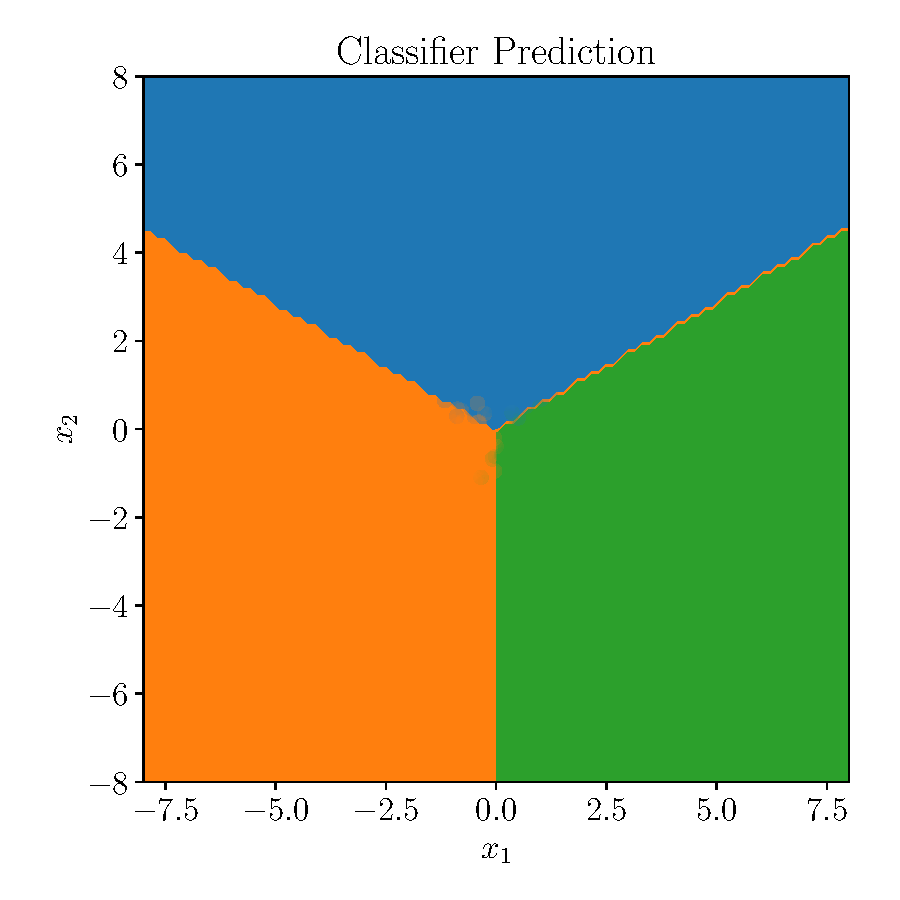
\includegraphics[width=\linewidth]{figures/toy_example/gaussian_mixture/classifier_class.pdf}
        \caption{}
        \label{fig:}
    \end{subfigure}
    % \hfill
    \begin{subfigure}[]{0.4\textwidth}
        \centering
        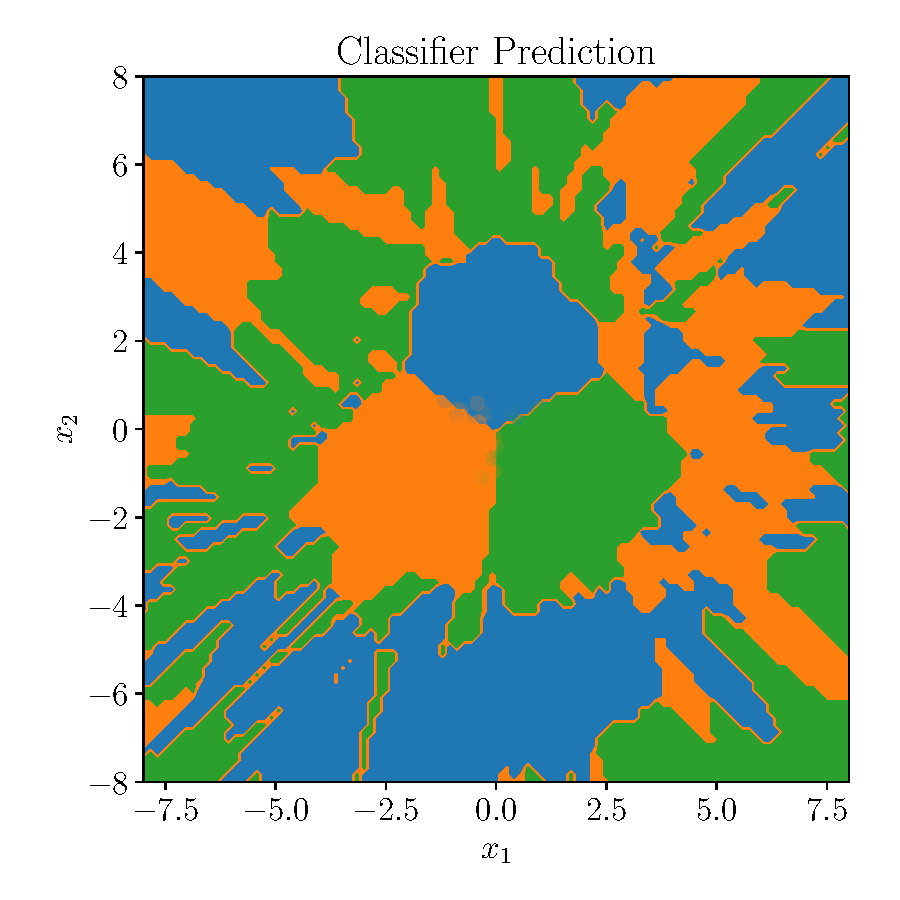
\includegraphics[width=\linewidth]{figures/toy_example/gaussian_mixture/classifier_kl_class.pdf}
        \caption{}
        \label{fig:}
    \end{subfigure}
    \begin{subfigure}[]{0.4\textwidth}
        \centering
    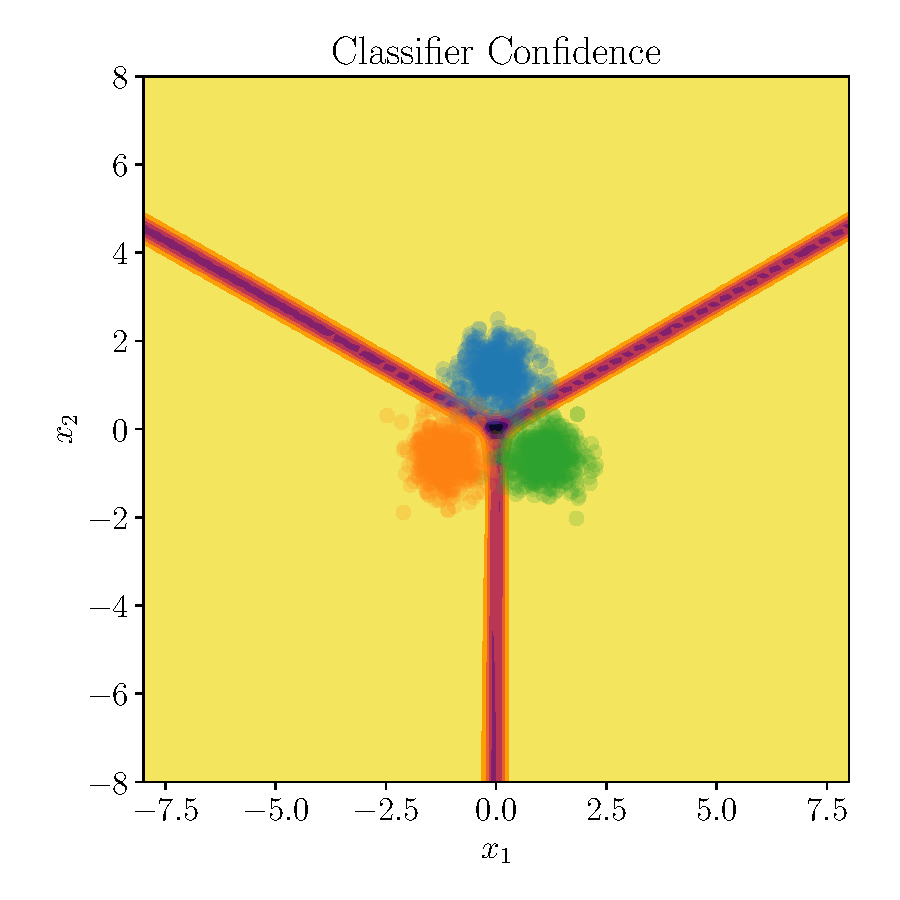
\includegraphics[width=\linewidth]{figures/toy_example/gaussian_mixture/classifier_confidence.pdf}
        \caption{}
        \label{fig:}
    \end{subfigure}
    \begin{subfigure}[]{0.4\textwidth}
        \centering
    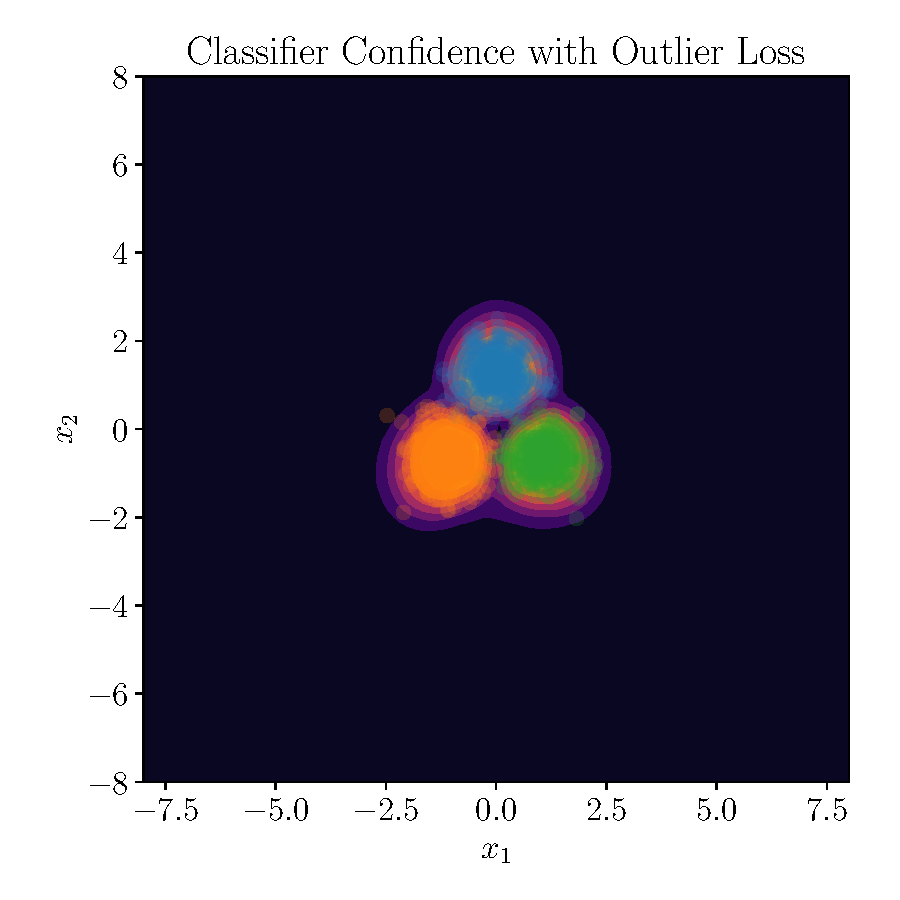
\includegraphics[width=\linewidth]{figures/toy_example/gaussian_mixture/classifier_kl_confidence.pdf}
        \caption{}
        \label{fig:}
    \end{subfigure}
    
    \caption{Gaussian mixture classifier performance}%
    \label{fig:classifier_gmm}
\end{figure}

\begin{figure}[htpb]
    \centering
    \begin{subfigure}[]{0.4\textwidth}
        \centering
    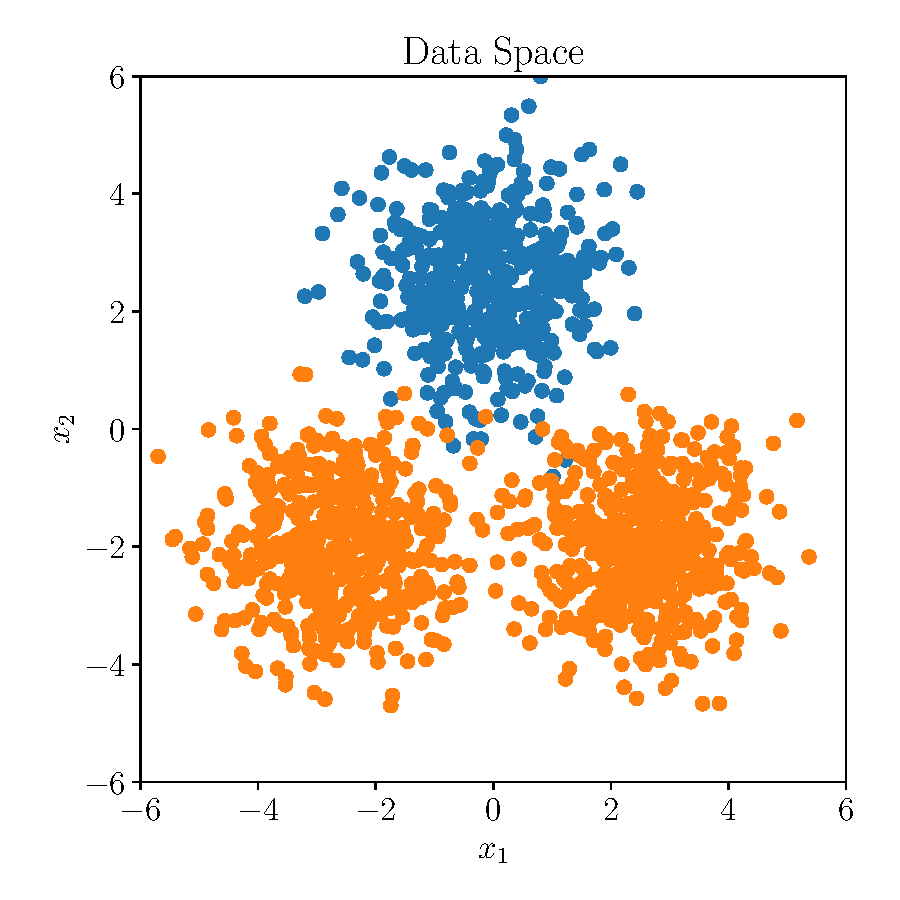
\includegraphics[width=\linewidth]{figures/toy_example/gaussian_mixture/toy_data.pdf}
        \caption{}
        \label{fig:}
    \end{subfigure}
    \begin{subfigure}[]{0.4\textwidth}
        \centering
    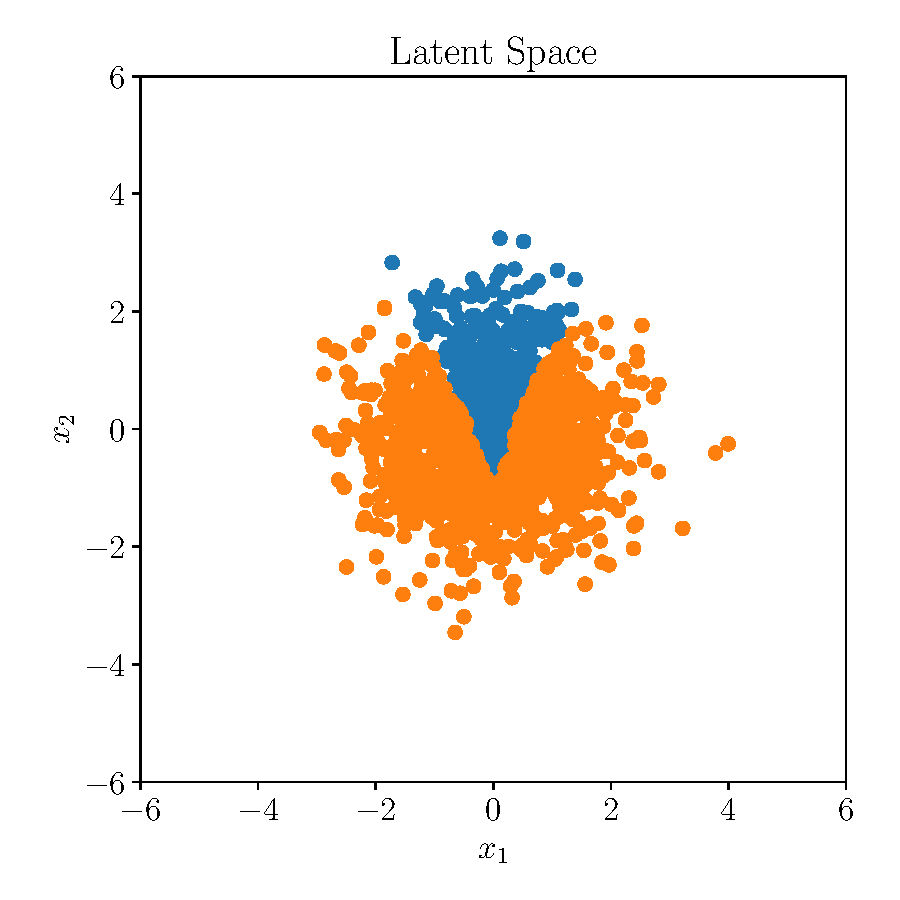
\includegraphics[width=\linewidth]{figures/toy_example/gaussian_mixture/latent_space.pdf}
        \caption{}
        \label{fig:}
    \end{subfigure}
    \begin{subfigure}[]{0.4\textwidth}
        \centering
    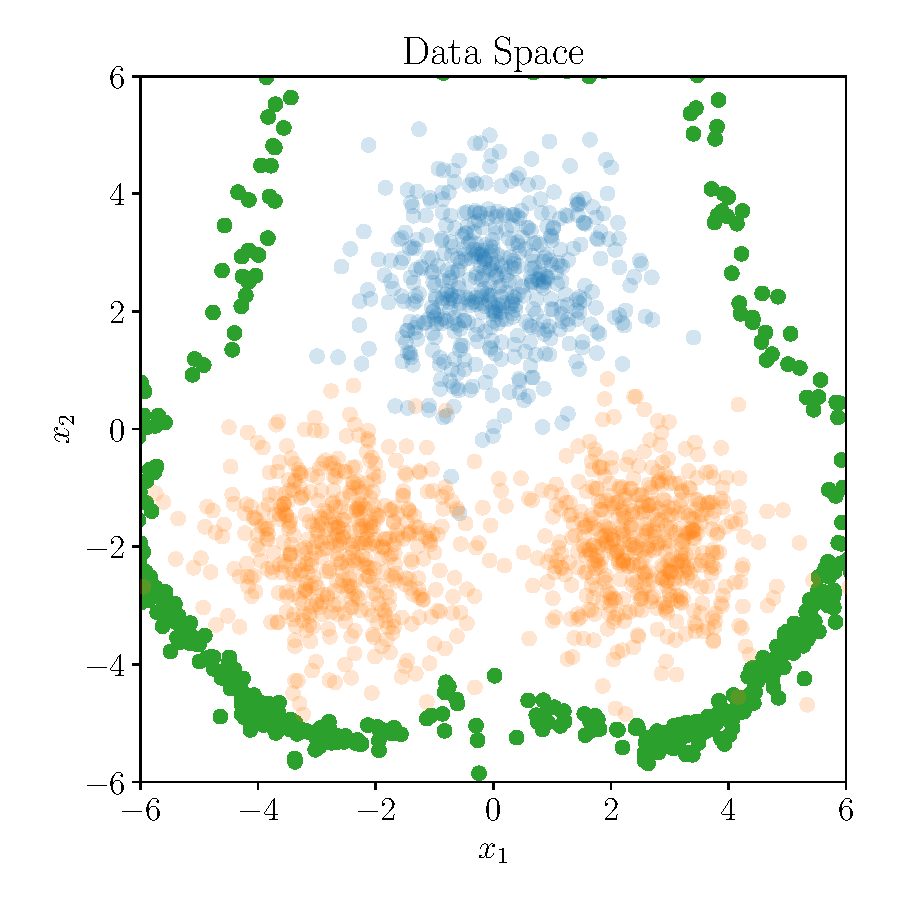
\includegraphics[width=\linewidth]{figures/toy_example/gaussian_mixture/gumbel_samples.pdf}
        \caption{}
        \label{fig:}
    \end{subfigure}
    \begin{subfigure}[]{0.4\textwidth}
        \centering
    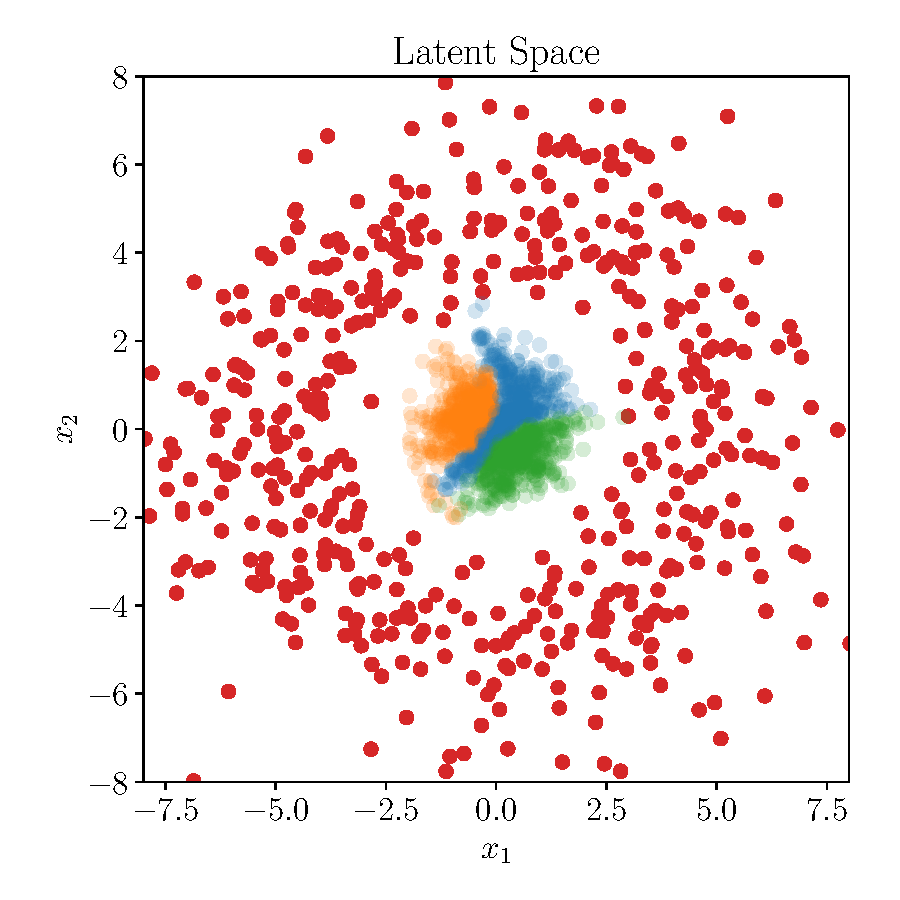
\includegraphics[width=\linewidth]{figures/toy_example/gaussian_mixture/latent_space_with_outliers.pdf}
        \caption{}
        \label{fig:}
    \end{subfigure}
    \caption{Gaussian mixture latent mapping}%
    \label{fig:latent_gmm}
\end{figure}

\begin{figure}[htpb]
    \centering
    \begin{subfigure}[]{0.4\textwidth}
        \centering
        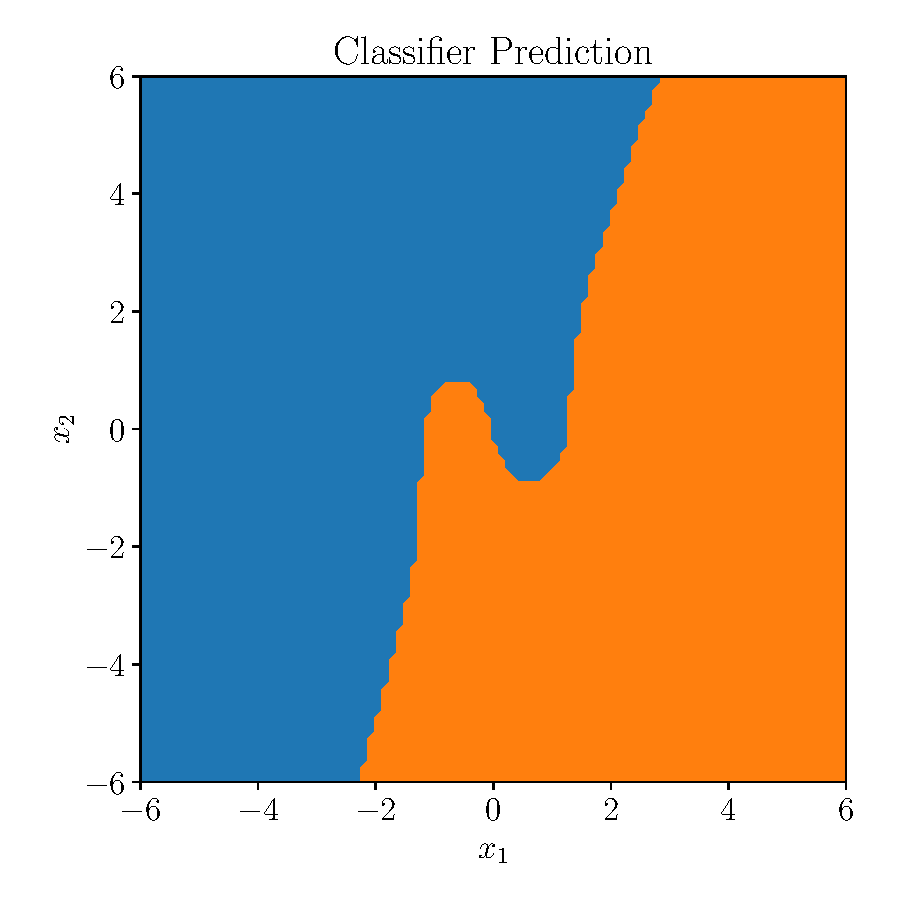
\includegraphics[width=\linewidth]{figures/toy_example/moons/classifier_class.pdf}
        \caption{}
        \label{fig:}
    \end{subfigure}
    % \hfill
    \begin{subfigure}[]{0.4\textwidth}
        \centering
        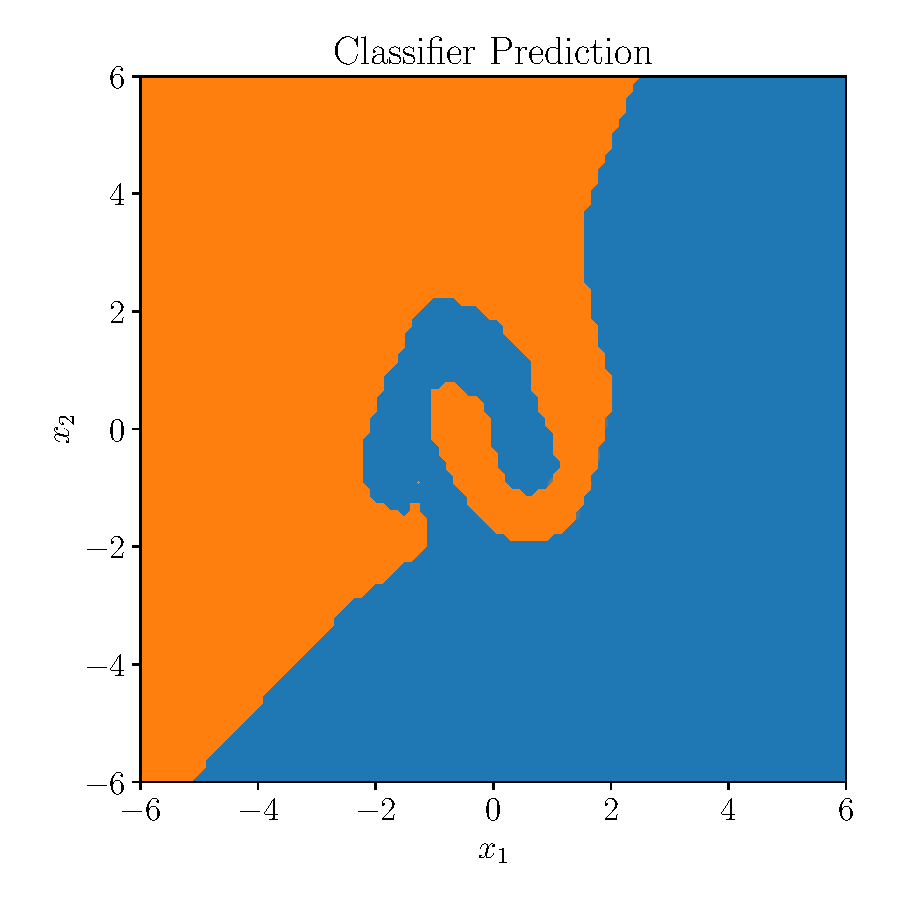
\includegraphics[width=\linewidth]{figures/toy_example/moons/classifier_kl_class.pdf}
        \caption{}
        \label{fig:}
    \end{subfigure}
    \begin{subfigure}[]{0.4\textwidth}
        \centering
    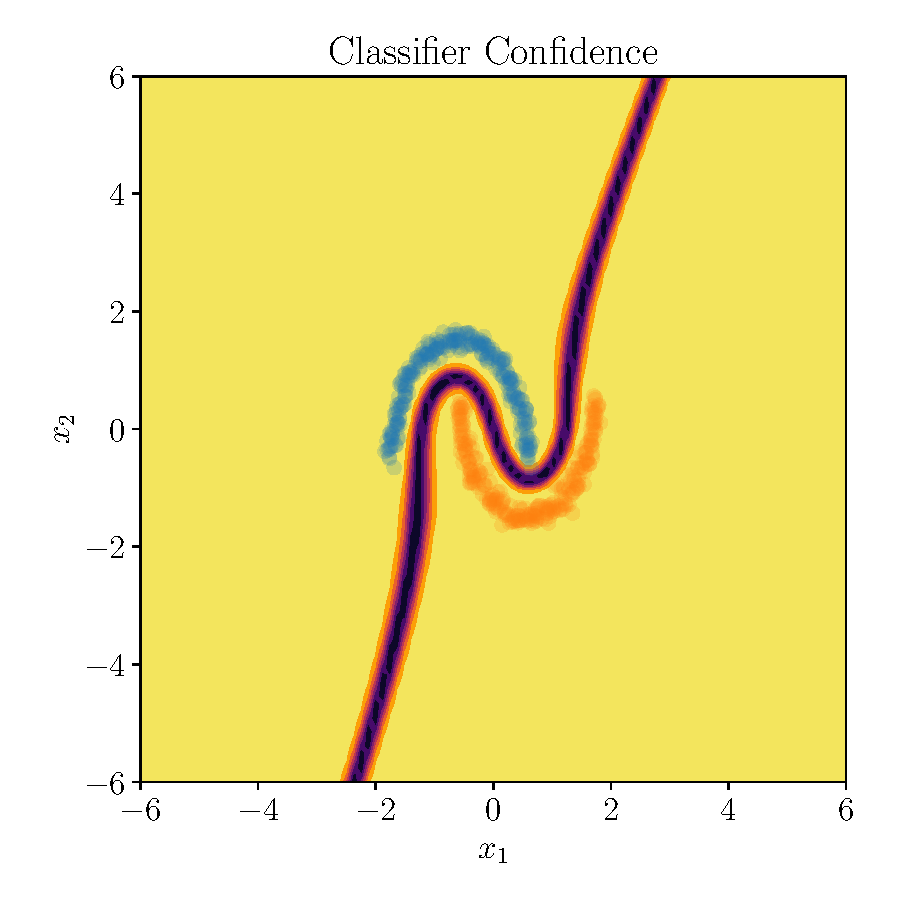
\includegraphics[width=\linewidth]{figures/toy_example/moons/classifier_confidence.pdf}
        \caption{}
        \label{fig:}
    \end{subfigure}
    \begin{subfigure}[]{0.4\textwidth}
        \centering
    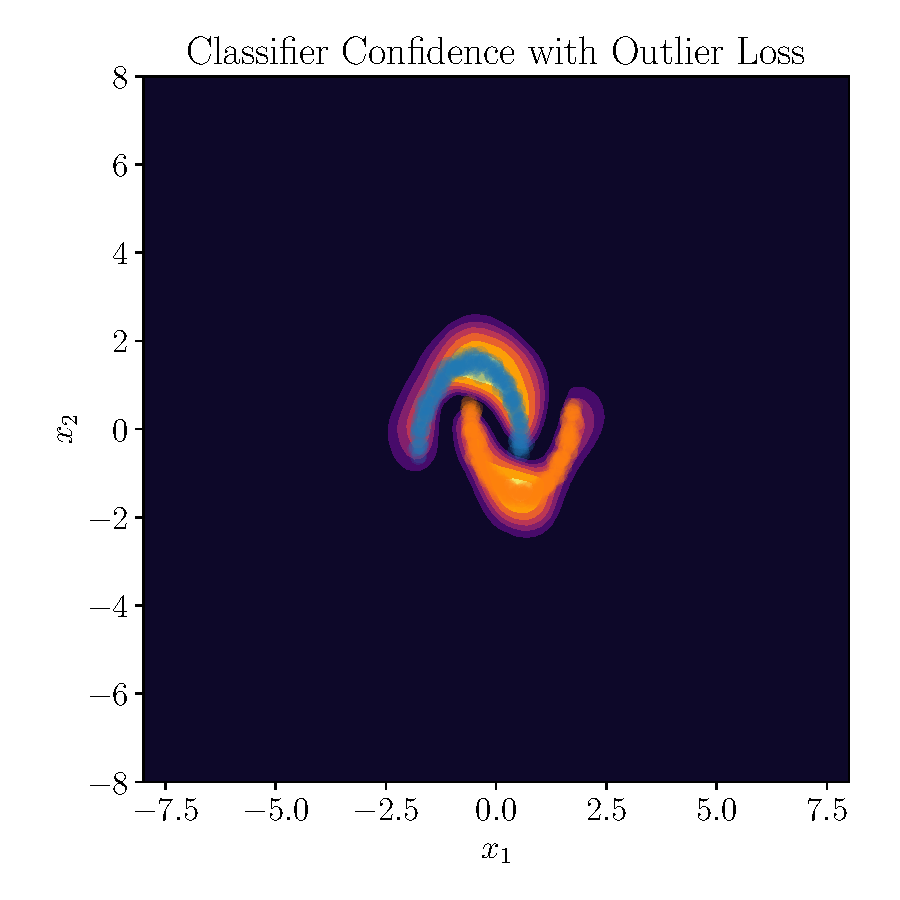
\includegraphics[width=\linewidth]{figures/toy_example/moons/classifier_kl_confidence.pdf}
        \caption{}
        \label{fig:}
    \end{subfigure}
    
    \caption{Moons classifier performance}%
    \label{fig:classifier_moons}
\end{figure}

\begin{figure}[htpb]
    \centering
    \begin{subfigure}[]{0.4\textwidth}
        \centering
    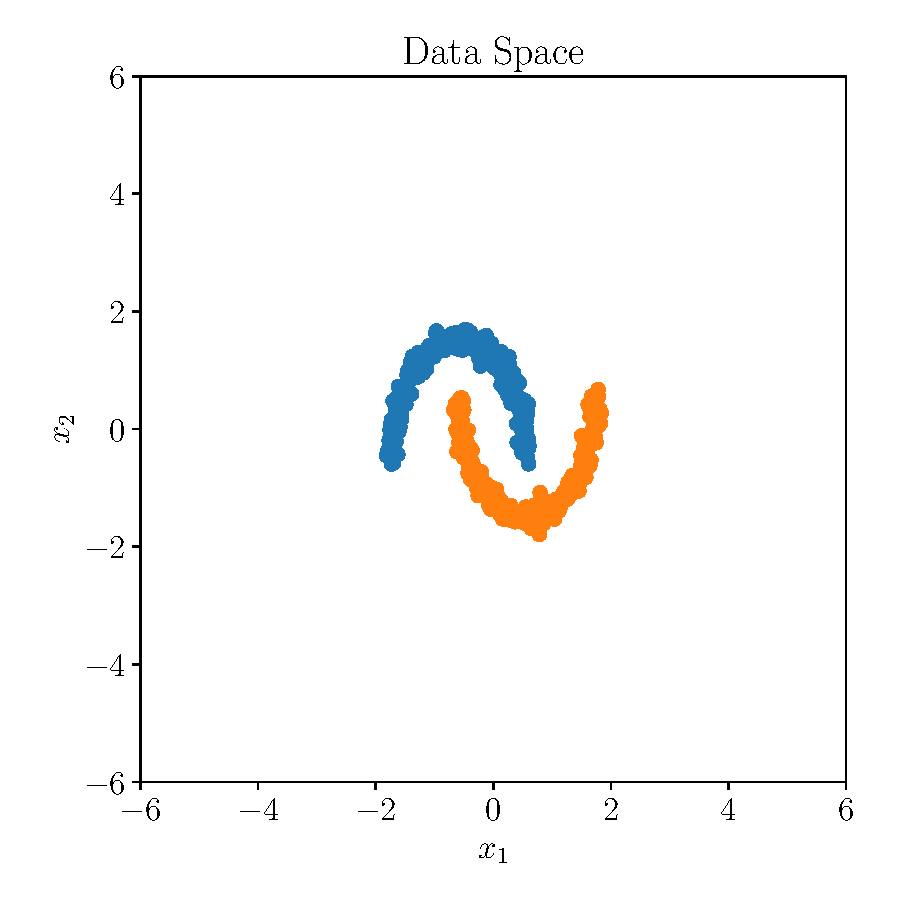
\includegraphics[width=\linewidth]{figures/toy_example/moons/toy_data.pdf}
        \caption{}
        \label{fig:}
    \end{subfigure}
    \begin{subfigure}[]{0.4\textwidth}
        \centering
    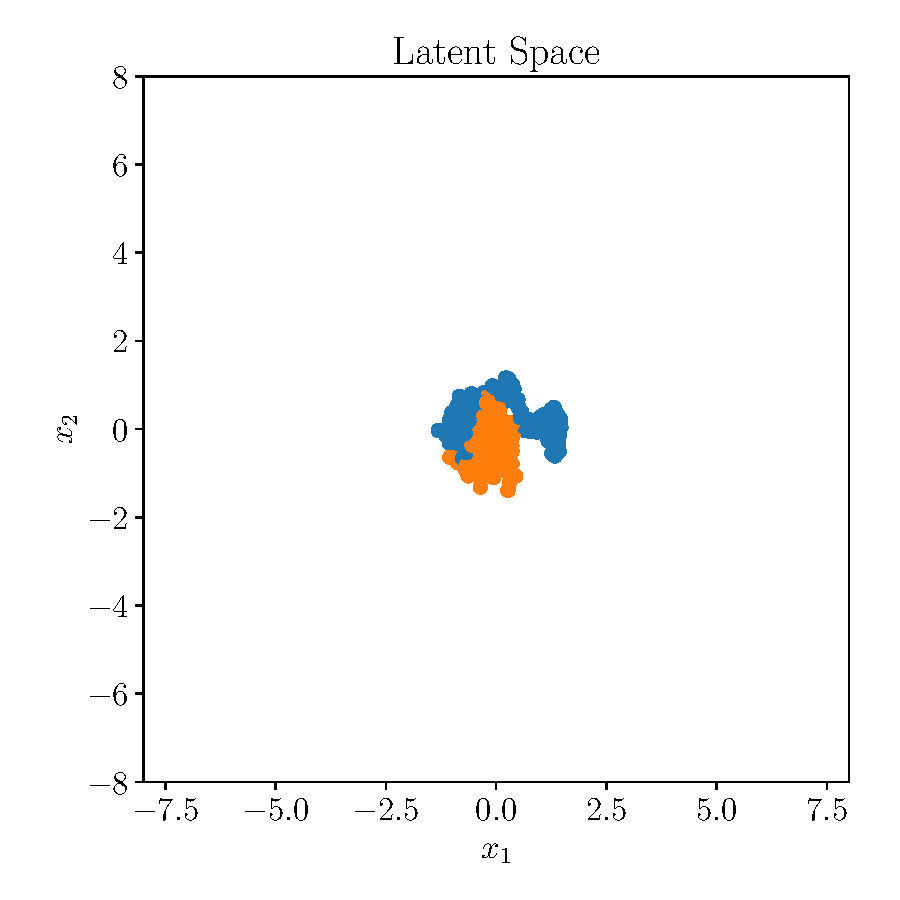
\includegraphics[width=\linewidth]{figures/toy_example/moons/latent_space.pdf}
        \caption{}
        \label{fig:}
    \end{subfigure}
    \begin{subfigure}[]{0.4\textwidth}
        \centering
    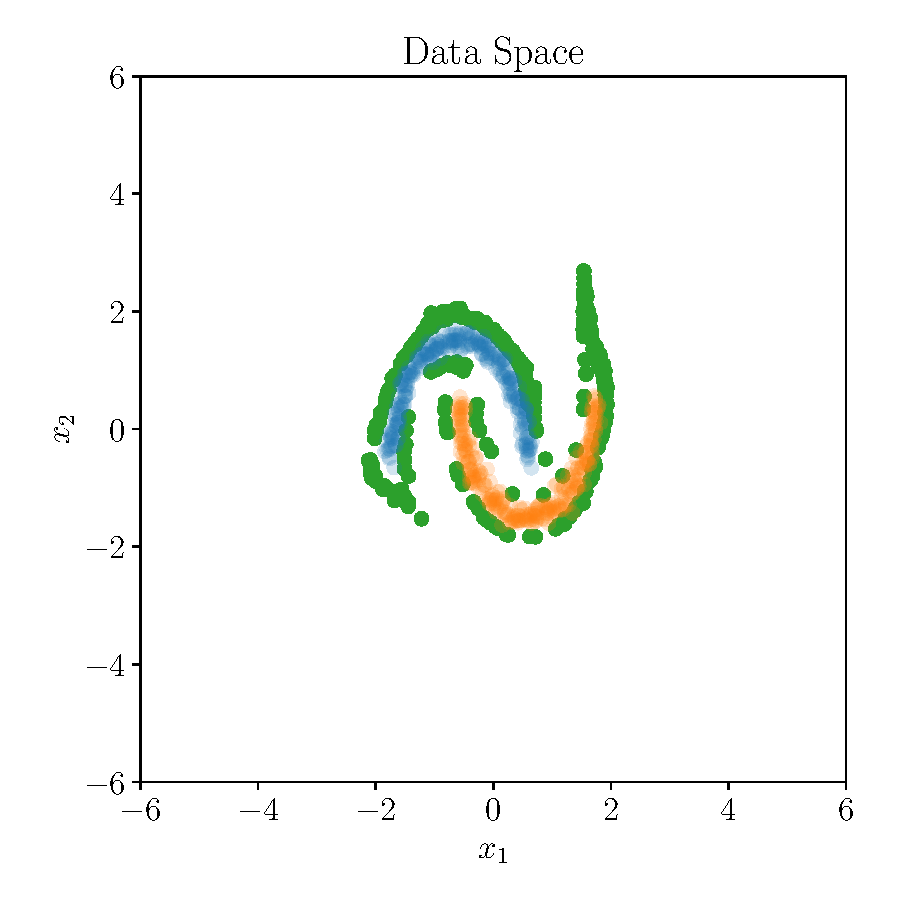
\includegraphics[width=\linewidth]{figures/toy_example/moons/gumbel_samples.pdf}
        \caption{}
        \label{fig:}
    \end{subfigure}
    \begin{subfigure}[]{0.4\textwidth}
        \centering
    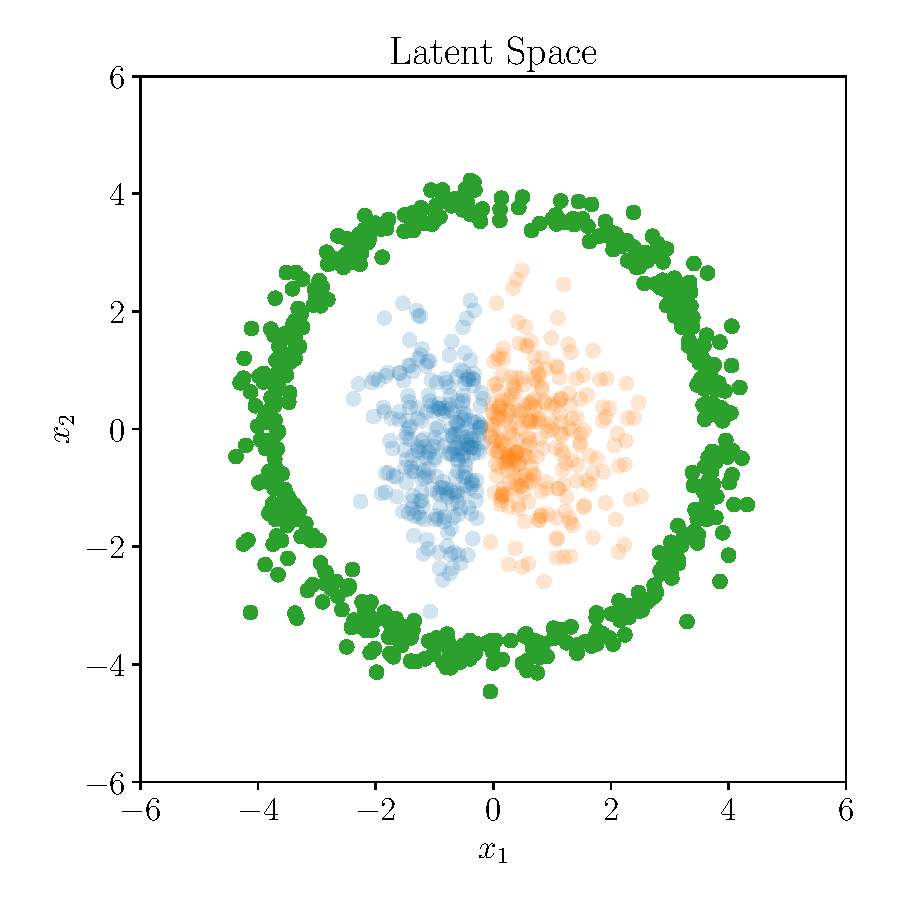
\includegraphics[width=\linewidth]{figures/toy_example/moons/latent_space_with_outliers.pdf}
        \caption{}
        \label{fig:}
    \end{subfigure}
    \caption{Moons latent mapping}%
    \label{fig:latent_moons}
\end{figure}

\section{Qualitative Comparison}%
\label{sec:qualitative_comparison}

\begin{figure}[htpb]
    \centering
    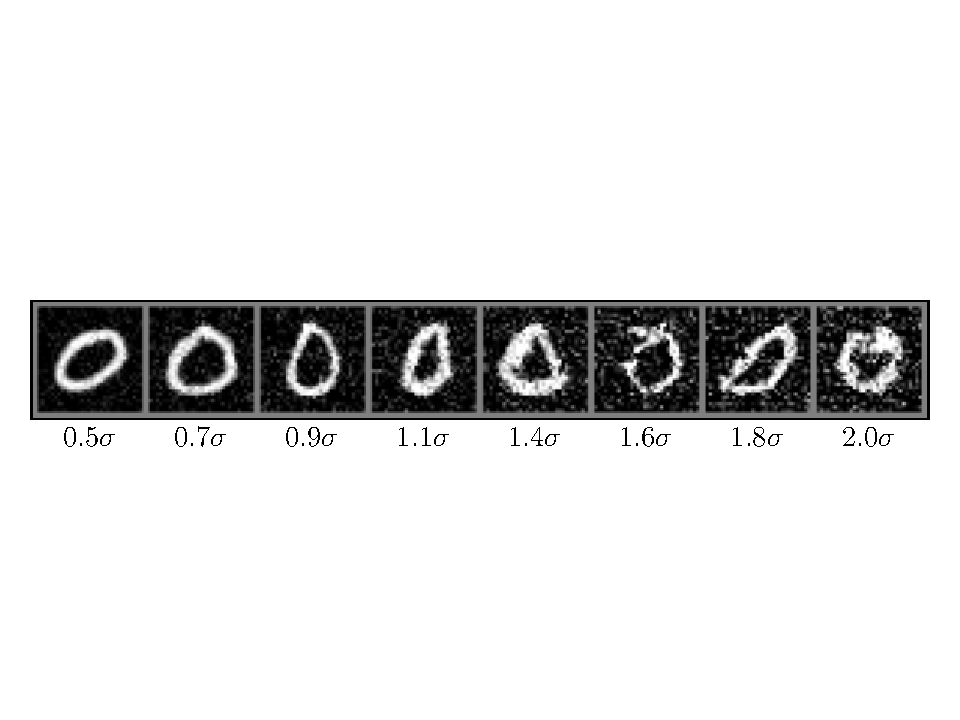
\includegraphics[width=0.8\linewidth]{figures/samples/emnist_inc_distance.pdf}
    \caption{}%
    \label{fig:}
\end{figure}

\begin{figure}[htpb]
    \centering
    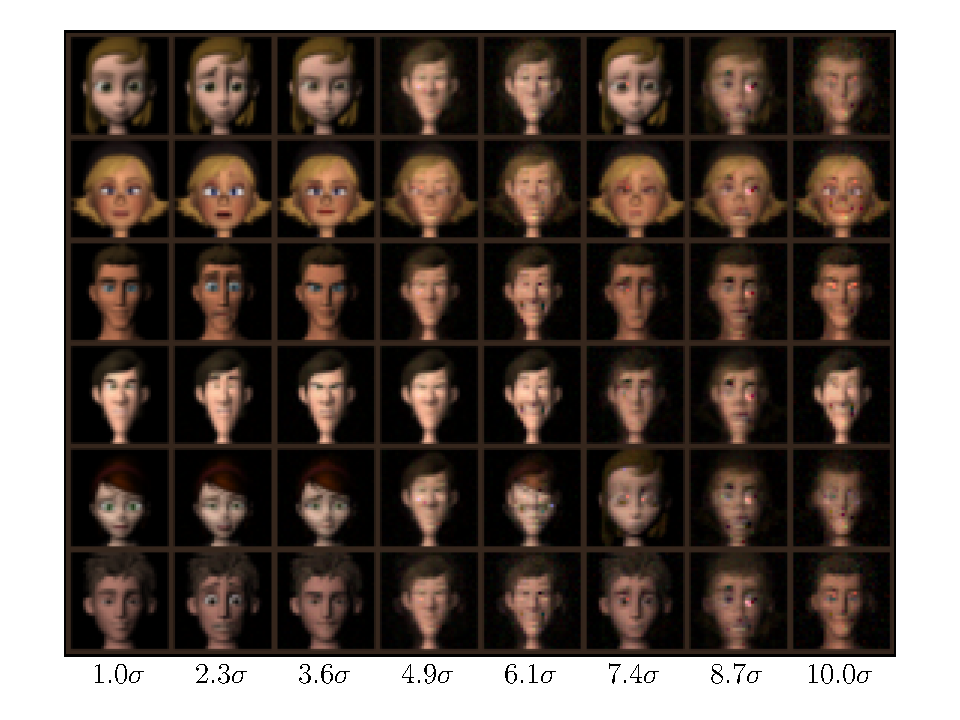
\includegraphics[width=0.8\linewidth]{figures/samples/ferg_people_inc_distance.pdf}
    \caption{}%
    \label{fig:}
\end{figure}

\subsection{Archetypal Analysis}%
\label{sub:archetypal_analysis}

\begin{figure}[htpb]
    \centering
    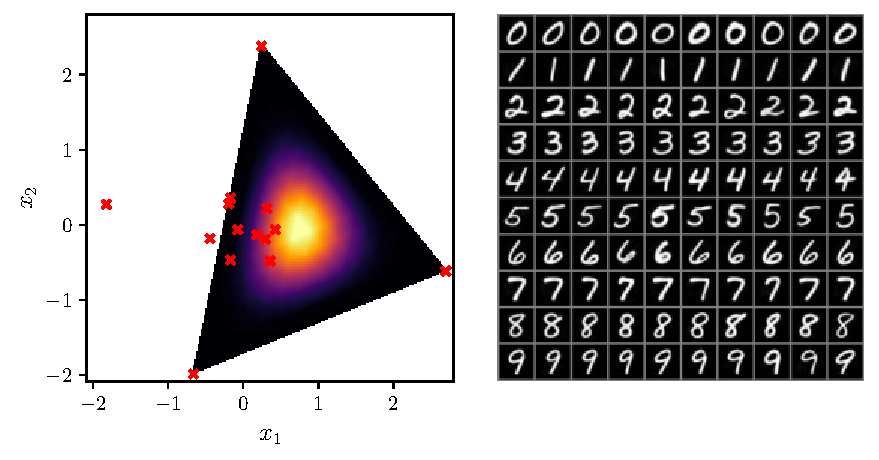
\includegraphics[width=1\linewidth]{figures/samples/aa_emnist.pdf}
    \caption{AA FERG}%
    \label{fig:aa_emnist}
\end{figure}

\begin{figure}[htpb]
    \centering
    \begin{subfigure}[htpb]{\textwidth}
        \centering
        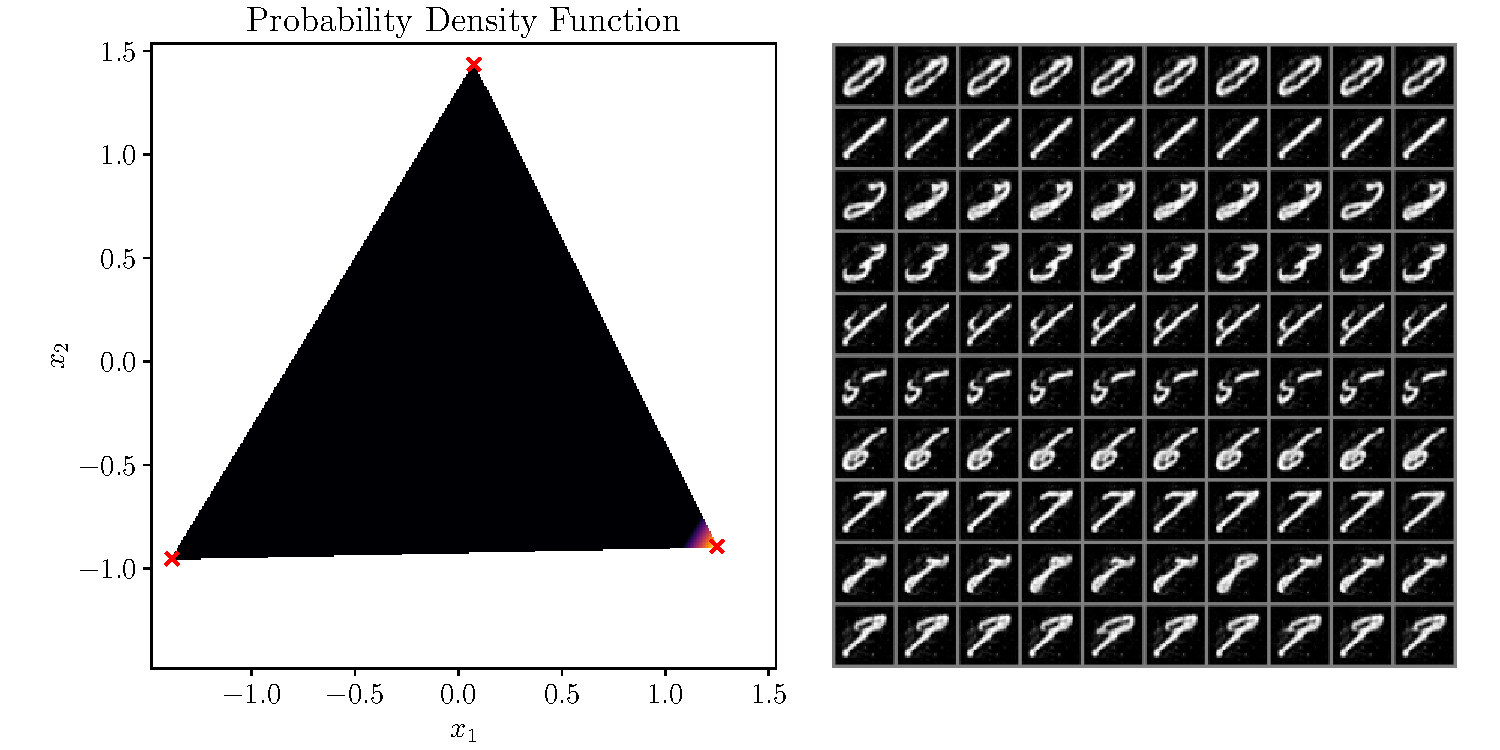
\includegraphics[width=1\linewidth]{figures/samples/aa_emnist1.pdf}
    \end{subfigure}

    \begin{subfigure}[htpb]{\textwidth}
        \centering
        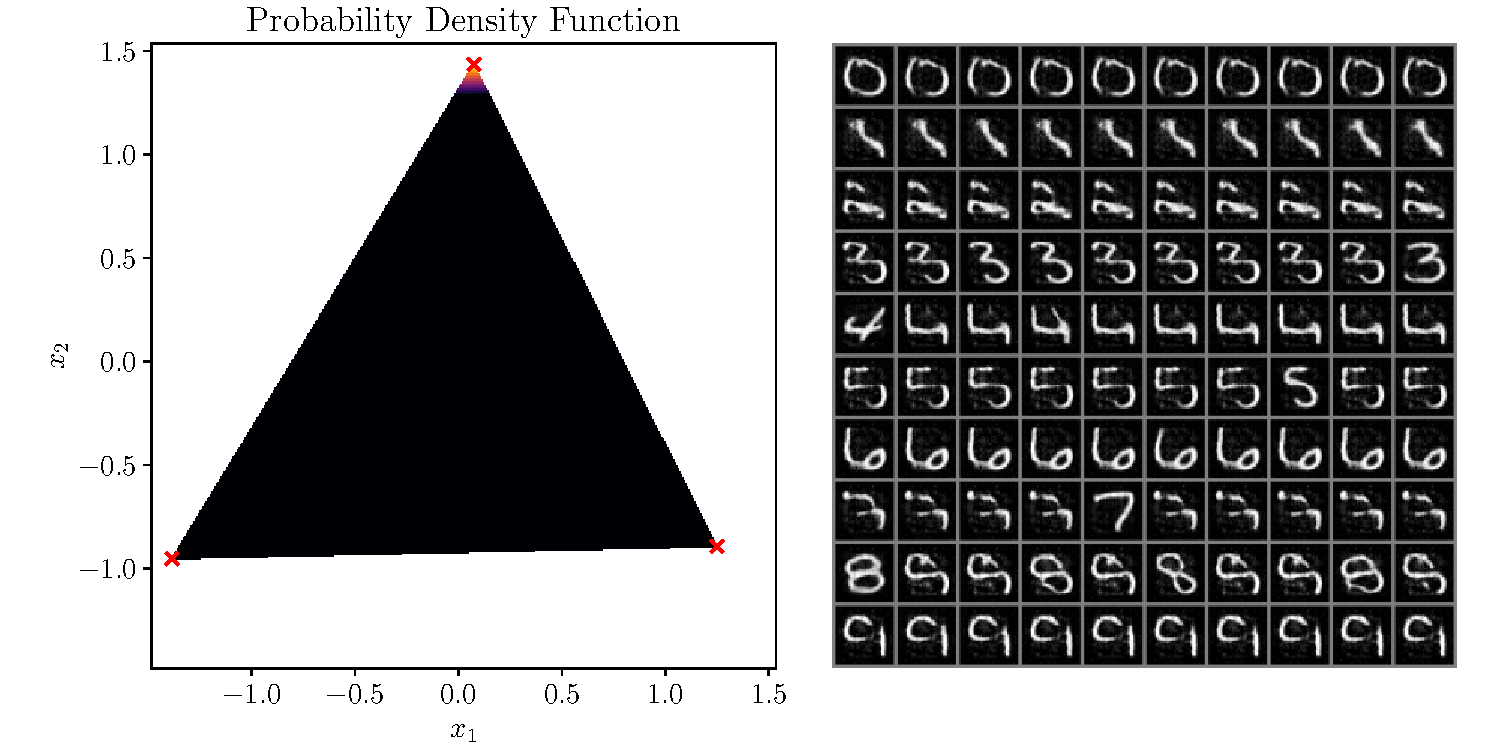
\includegraphics[width=1\linewidth]{figures/samples/aa_emnist2.pdf}
    \end{subfigure}

    \begin{subfigure}[htpb]{\textwidth}
        \centering
        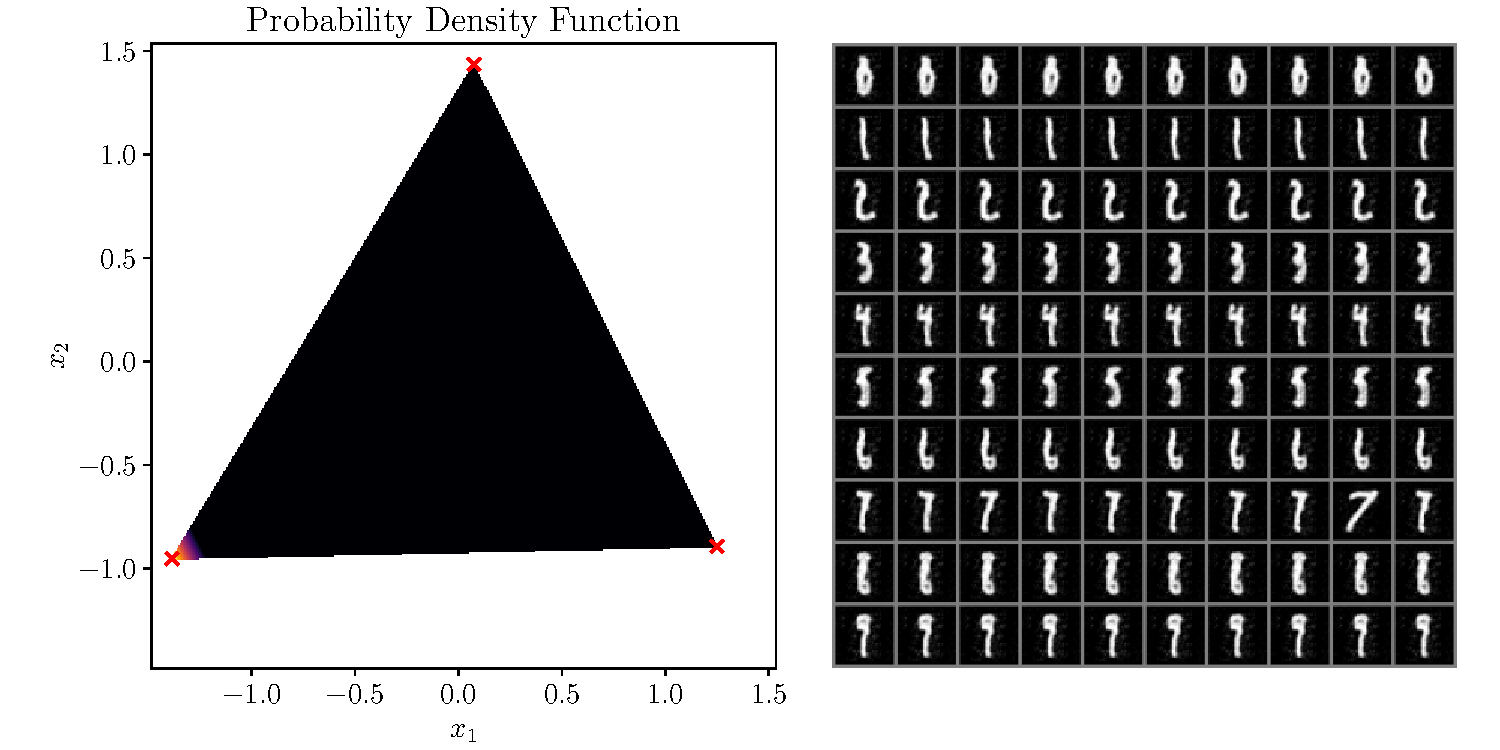
\includegraphics[width=1\linewidth]{figures/samples/aa_emnist3.pdf}
    \end{subfigure}
    \caption{Name}%
    \label{fig:name}
\end{figure}

\begin{figure}[htpb]
    \centering
    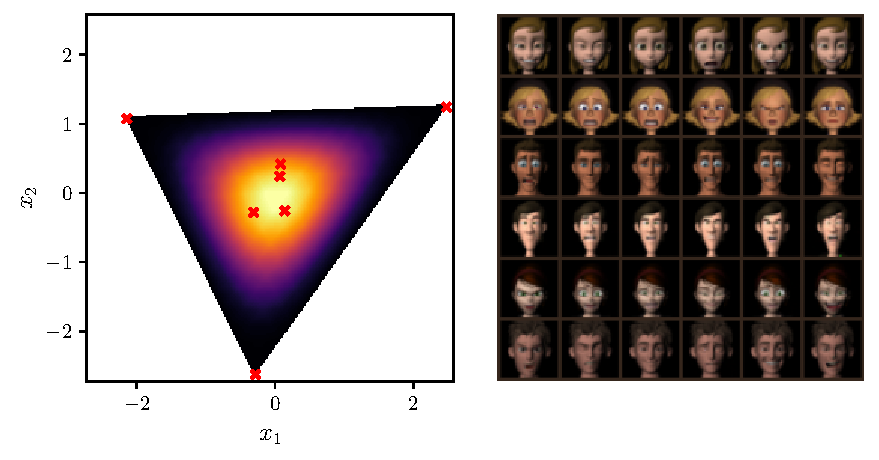
\includegraphics[width=1\linewidth]{figures/samples/aa_ferg.pdf}
    \caption{AA FERG}%
    \label{fig:aa_ferg}
\end{figure}

\begin{figure}[htpb]
    \centering
    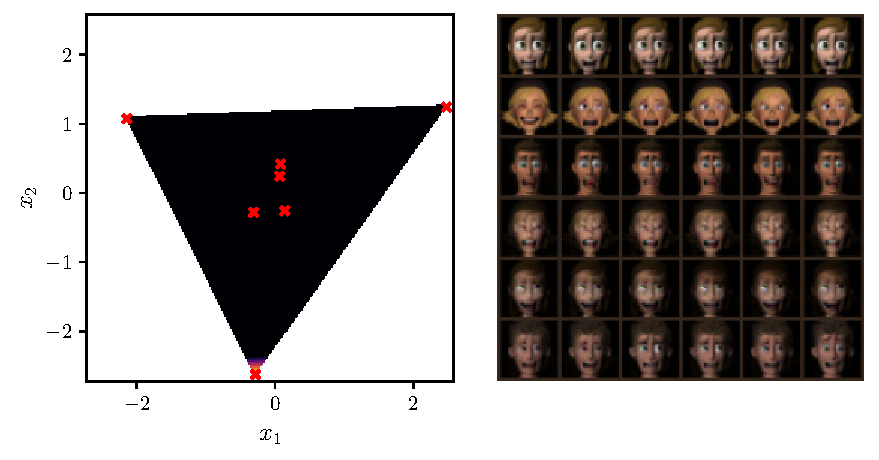
\includegraphics[width=1\linewidth]{figures/samples/aa_ferg1.pdf}
    \caption{AA FERG}%
    \label{fig:aa_ferg}
\end{figure}

\begin{figure}[htpb]
    \centering
    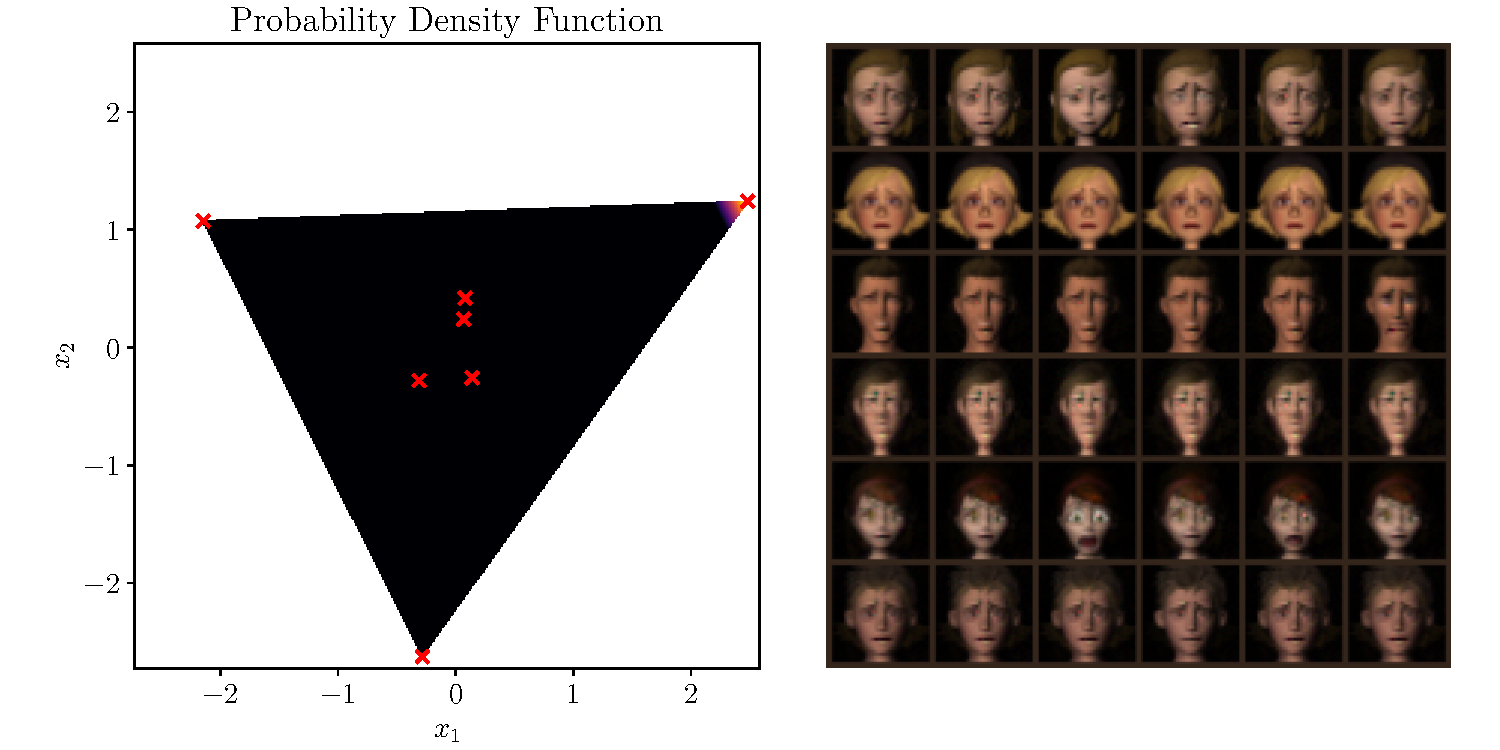
\includegraphics[width=1\linewidth]{figures/samples/aa_ferg2.pdf}
    \caption{AA FERG}%
    \label{fig:aa_ferg}
\end{figure}

\begin{figure}[htpb]
    \centering
    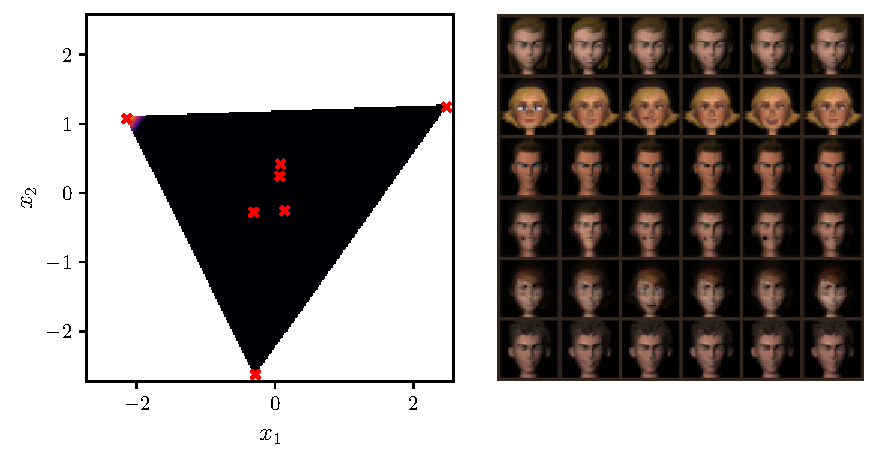
\includegraphics[width=1\linewidth]{figures/samples/aa_ferg3.pdf}
    \caption{AA FERG}%
    \label{fig:aa_ferg}
\end{figure}


\section{Discriminator Performance}%
\label{sec:discriminator_performance}


\section{Analysis of the Latent Space}%
\label{sec:analysis_of_the_latent_space}

\begin{figure}[htpb]
    \centering
    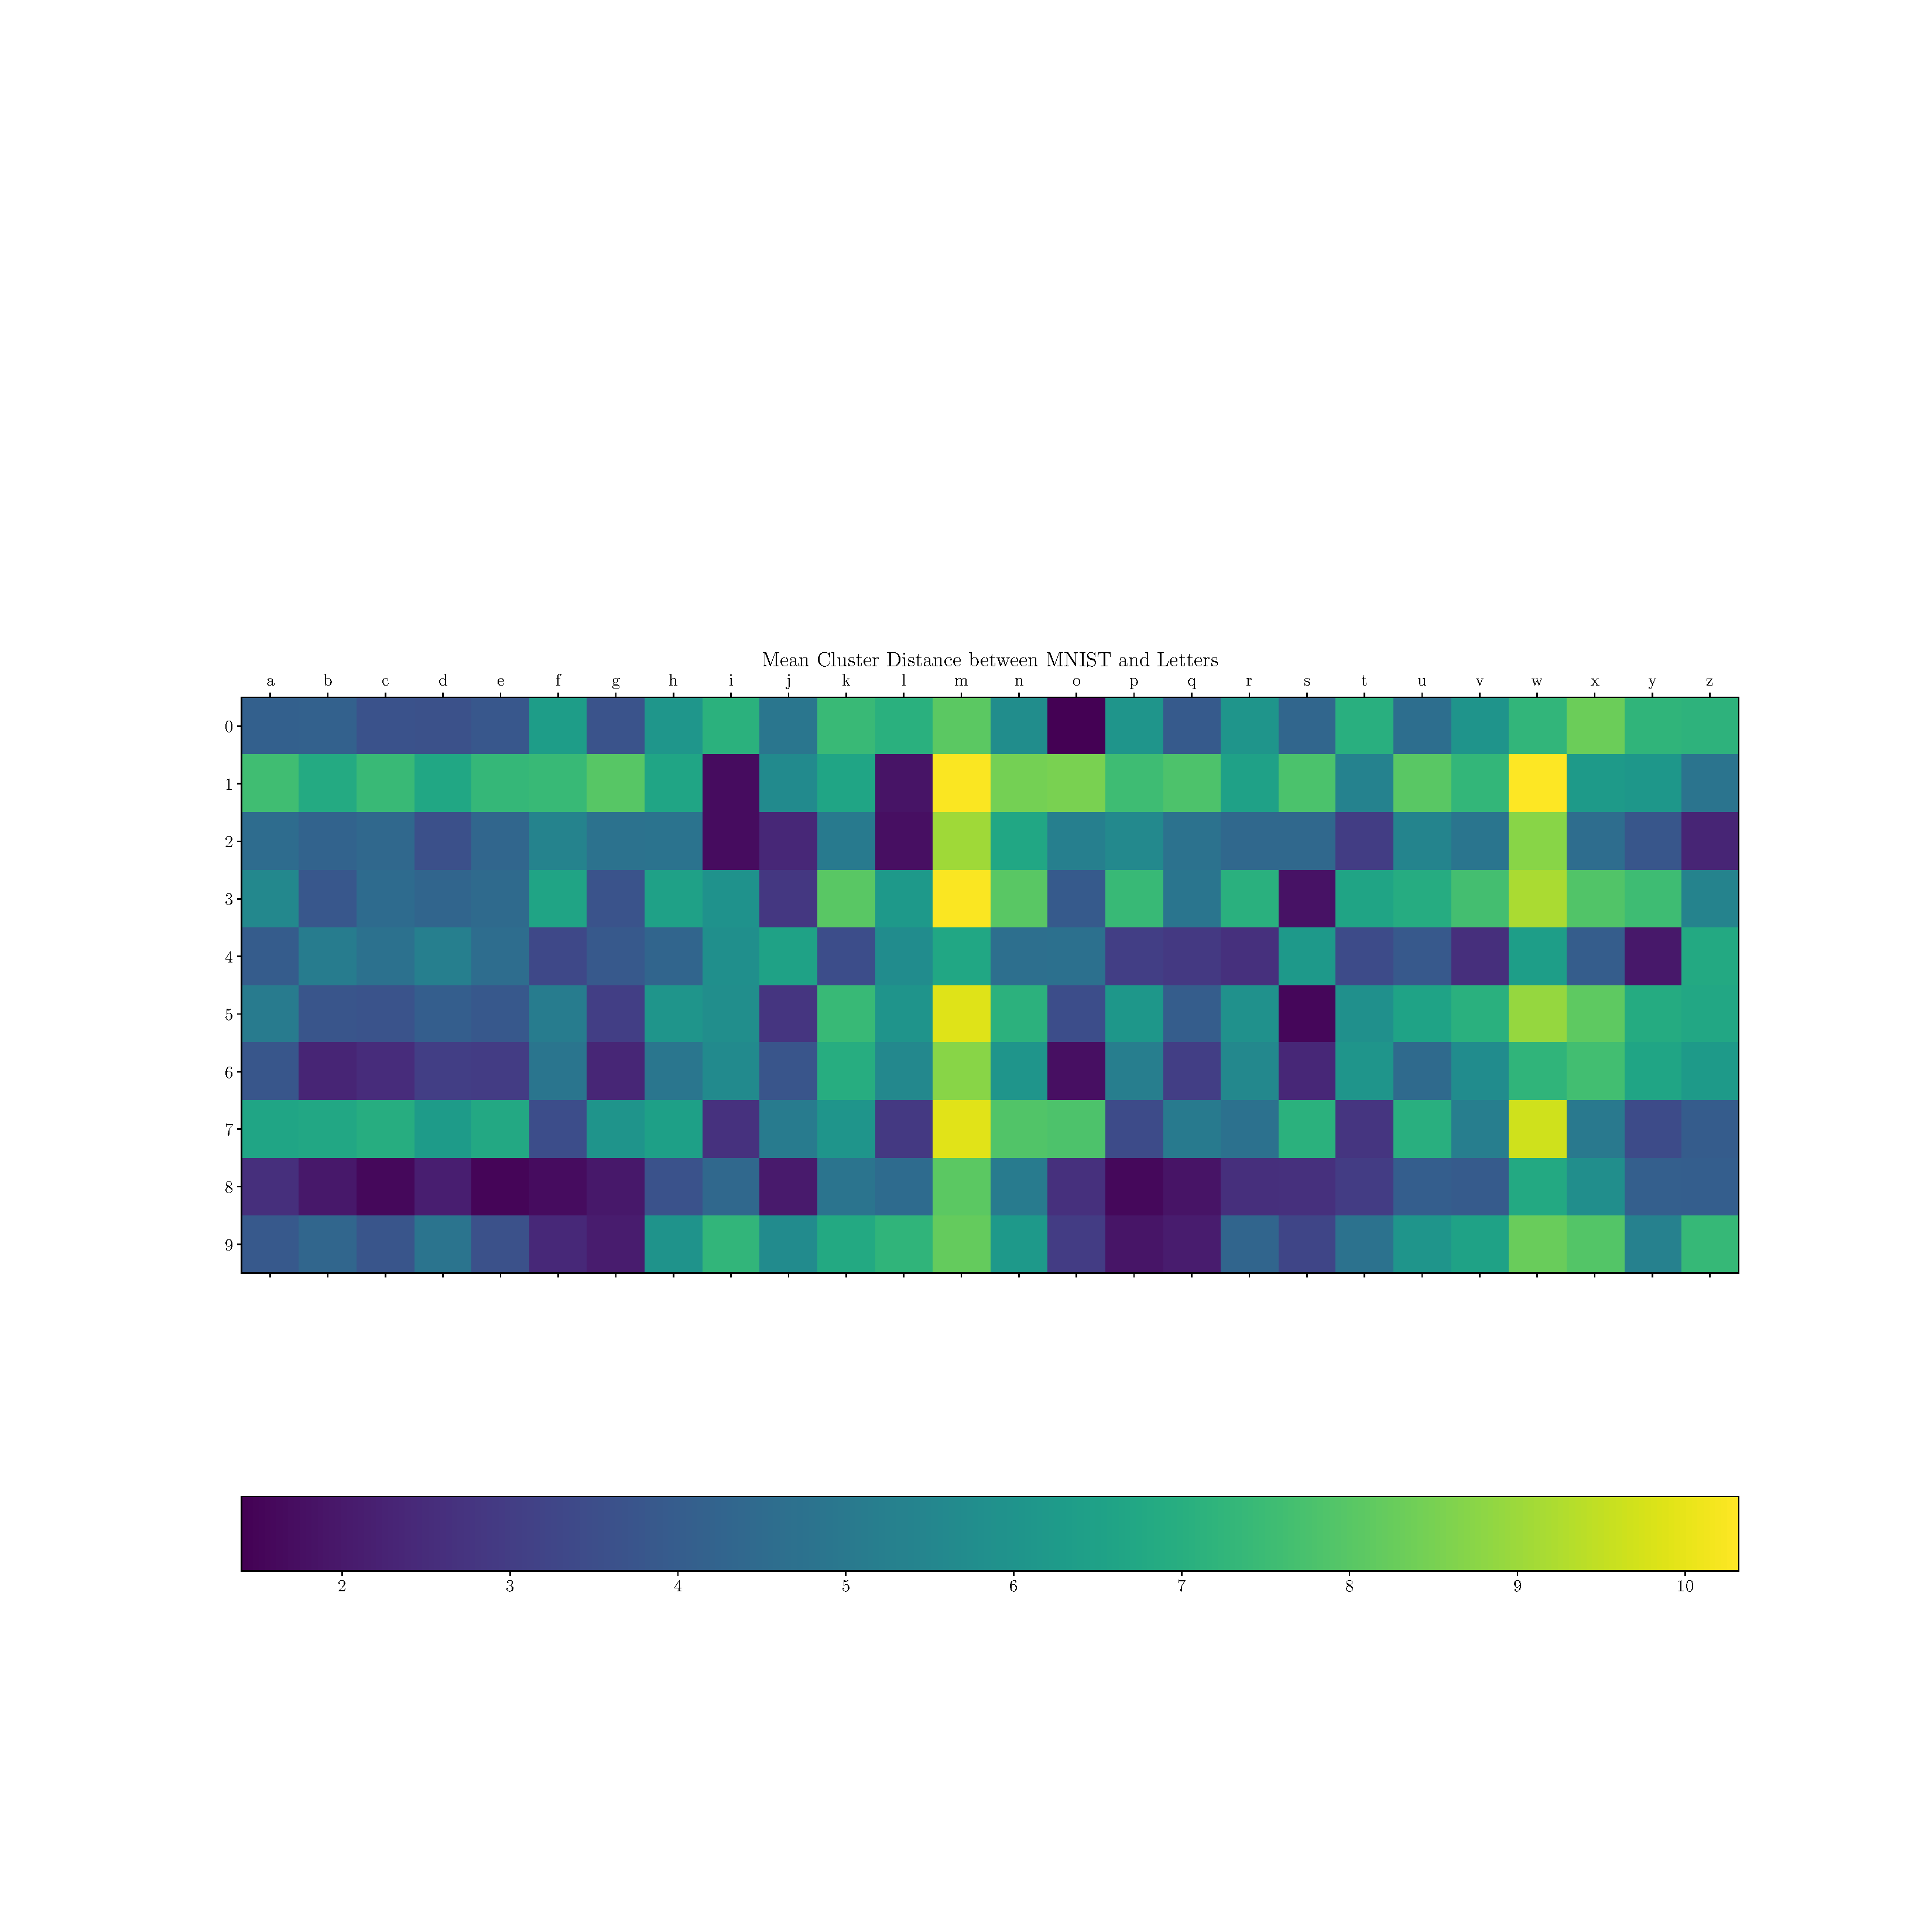
\includegraphics[width=0.8\linewidth]{figures/samples/emnist_distance_matrix_letters.pdf}
    \caption{}%
    \label{fig:}
\end{figure}

\begin{figure}[htpb]
    \centering
    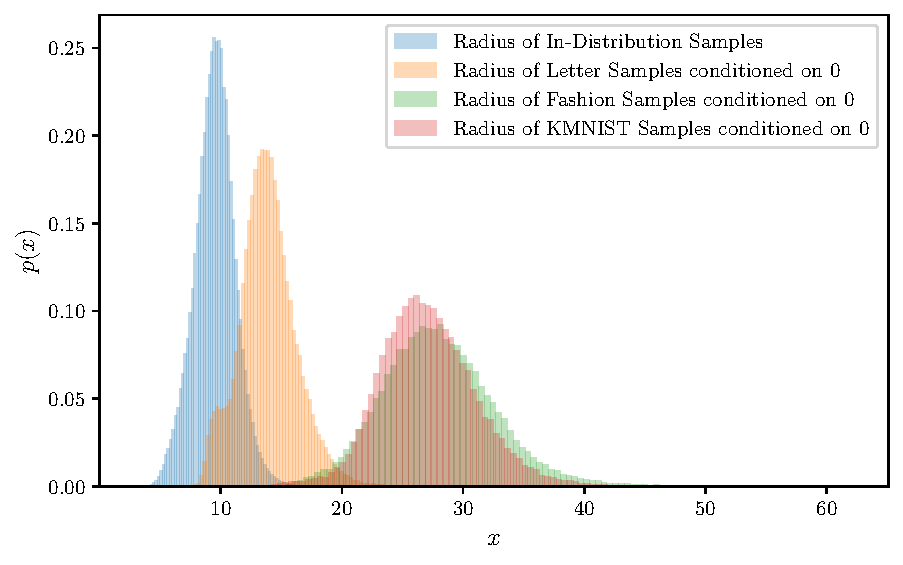
\includegraphics[width=0.8\linewidth]{figures/samples/emnist_radius_hist.pdf}
    \caption{}%
    \label{fig:}
\end{figure}


\section{General Performance}%
\label{sec:general_performance}

% What did I even mean by this?

\section{Robustness}%
\label{sec:robustness}

% If there is time for this

% TODO: Check if anything Ulli requested isn't done yet %
